\documentclass[10pt]{article}

\usepackage{enumerate}
\usepackage{amsmath}
\usepackage{amssymb}
\usepackage{amsthm}
\usepackage{array}
\usepackage[all]{xy}
\usepackage{fancyhdr}
\usepackage{euscript}
\usepackage{graphics}
\usepackage{cancel}
\usepackage{fancybox}
\usepackage{tikz}
\usepackage{tikz-3dplot}
\usepackage{pgf}
\usepackage{pgfplots}
\usepackage[all]{xy}
\usepackage{graphicx}
\pgfplotsset{compat=1.14}

\usepackage{pstricks}
\usepackage{pst-plot}

\usepackage{setspace}
\onehalfspacing

\setlength{\oddsidemargin}{.5in}
\setlength{\evensidemargin}{.5in}
\setlength{\textwidth}{6.in}
\setlength{\topmargin}{0in}
\setlength{\headsep}{.20in}
\setlength{\textheight}{8.5in}


\pdfpagewidth 8.5in
 \pdfpageheight 11in


%General
\newcommand{\WW}{\mathbb {W}}
\newcommand{\ZZ}{\mathbb{Z}}
\newcommand{\RR}{\mathbb {R}}
\newcommand{\II}{\mathbb {I}}
\newcommand{\QQ}{\mathbb {Q}}
\newcommand{\CC}{\mathbf C}
\newcommand{\NN}{\mathbb {N}}
\newcommand{\Zn}[1]{\mathbf{Z}/#1\mathbf{Z}}
\newcommand{\Znx}[1]{(\mathbf{Z}/#1\mathbf{Z})^\times}
\newcommand{\X}{\times} 
\newcommand{\set}[2]{\left\{#1 : #2\right\}}          
\newcommand{\sett}[1]{\left\{#1\right\}}                
\newcommand{\nonempty}{\neq\varnothing}
\newcommand{\ds}{\displaystyle}
\newcommand{\abs}[1]{\left| {#1} \right|}
\newcommand{\qedbox}{\rule{2mm}{2mm}}
\renewcommand{\qedsymbol}{\qedbox}											
\newcommand{\aand}{\qquad\hbox{and}\qquad}
\newcommand{\e}{\varepsilon}
\newcommand{\tto}{\rightrightarrows}
\newcommand{\gs}{\geqslant}
\newcommand{\ls}{\leqslant}
\renewcommand{\tilde}{\widetilde}
\renewcommand{\hat}{\widehat}
\newcommand{\norm}[1]{\left\| #1 \right\|}
\newcommand{\md}[3]{#1\equiv#2\;(\mathrm{mod}\;#3)}     
\newcommand{\gen}[1]{\left\langle #1 \right\rangle}
\renewcommand{\Re}{\operatorname{Re}}
\renewcommand{\Im}{\operatorname{Im}}
\newcommand{\zero}{\boldsymbol{0}}

\newcommand{\be}[1]{\textbf{\emph{#1}}}
\newcommand{\hhat}[1]{\hat{\! \hat{#1}}}

\newcommand{\fto}[1]{\xrightarrow{\hspace{4pt} #1 \hspace{4pt}}}
\newcommand{\flto}[1]{\xrightarrow{\quad #1 \quad}}



\newcommand{\dist}{\operatorname{dist}}
\newcommand{\esssup}{\operatorname{ess\:sup}}
\newcommand{\id}{\operatorname{id}}
\newcommand{\card}{\operatorname{card}}

\newcommand{\dmu}{\:\mathrm{d}\mu}
\newcommand{\dm}{\:\mathrm{d}m}
\newcommand{\dx}{\:\mathrm{d}x}
\newcommand{\dt}{\:\mathrm{d}t}
\newcommand{\dz}{\:\mathrm{d}z}
\newcommand{\dtheta}{\:\mathrm{d}\theta}
\newcommand{\dw}{\:\mathrm{d}w}

%Algebra
\newcommand{\Sym}{\operatorname {Sym}}
\newcommand{\Stab}{\operatorname {Stab}}
\newcommand{\M}{\operatorname{M}}
\newcommand{\GL}{\operatorname{GL}}
\newcommand{\PGL}{\operatorname{PGL}}
\newcommand{\SL}{\operatorname{SL}}
\newcommand{\PSL}{\operatorname{PSL}}
\newcommand{\Heis}{\operatorname{Heis}}
\newcommand{\Aff}{\operatorname{Aff}}
\newcommand{\Aut}{\operatorname{Aut}}
\newcommand{\image}{\operatorname{im}}
\newcommand{\Syl}[2]{\operatorname{\emph{Syl}}_{#1}\left(#2\right)}
\newcommand{\Hom}{\operatorname{Hom}}
\newcommand{\Tor}{\operatorname{Tor}}
\newcommand{\Gal}{\operatorname{Gal}}
\newcommand{\ch}{\operatorname{ch}}
\newcommand{\rad}{\operatorname{rad}}
\newcommand{\iso}{\cong}
\newcommand{\normal}{\unlhd}
\newcommand{\semi}{\rtimes}
\newcommand{\Nm}{\operatorname {N}}
\newcommand{\Tr}{\operatorname {Tr}}
\newcommand{\disc}{\operatorname {disc}}








%Euler Script Characters
\newcommand{\esa}{\EuScript{A}}
\newcommand{\esb}{\EuScript{B}}
\newcommand{\esc}{\EuScript{C}}
\newcommand{\esd}{\EuScript{D}}
\newcommand{\ese}{\EuScript{E}}
\newcommand{\esf}{\EuScript{F}}
\newcommand{\esg}{\EuScript{G}}
\newcommand{\esh}{\EuScript{H}}
\newcommand{\esi}{\EuScript{I}}
\newcommand{\esj}{\EuScript{J}}
\newcommand{\esk}{\EuScript{K}}
\newcommand{\esl}{\EuScript{L}}
\newcommand{\esm}{\EuScript{M}}
\newcommand{\esn}{\EuScript{N}}
\newcommand{\eso}{\EuScript{O}}
\newcommand{\esp}{\EuScript{P}}
\newcommand{\esq}{\EuScript{Q}}
\newcommand{\esr}{\EuScript{R}}
\newcommand{\ess}{\EuScript{S}}
\newcommand{\est}{\EuScript{T}}
\newcommand{\esu}{\EuScript{U}}
\newcommand{\esv}{\EuScript{V}}
\newcommand{\esw}{\EuScript{W}}
\newcommand{\esx}{\EuScript{X}}
\newcommand{\esy}{\EuScript{Y}}
\newcommand{\esz}{\EuScript{Z}}

%Calligraphic Characters
\newcommand{\cala}{\mathcal{A}}
\newcommand{\calb}{\mathcal{B}}
\newcommand{\calc}{\mathcal{C}}
\newcommand{\cald}{\mathcal{D}}
\newcommand{\cale}{\mathcal{E}}
\newcommand{\calf}{\mathcal{F}}
\newcommand{\calg}{\mathcal{G}}
\newcommand{\calh}{\mathcal{H}}
\newcommand{\cali}{\mathcal{I}}
\newcommand{\calj}{\mathcal{J}}
\newcommand{\calk}{\mathcal{K}}
\newcommand{\call}{\mathcal{L}}
\newcommand{\calm}{\mathcal{M}}
\newcommand{\caln}{\mathcal{N}}
\newcommand{\calo}{\mathcal{O}}
\newcommand{\calp}{\mathcal{P}}
\newcommand{\calq}{\mathcal{Q}}
\newcommand{\calr}{\mathcal{R}}
\newcommand{\cals}{\mathcal{S}}
\newcommand{\calt}{\mathcal{T}}
\newcommand{\calu}{\mathcal{U}}
\newcommand{\calv}{\mathcal{V}}
\newcommand{\calw}{\mathcal{W}}
\newcommand{\calx}{\mathcal{X}}
\newcommand{\caly}{\mathcal{Y}}
\newcommand{\calz}{\mathcal{Z}}

%Gothic Characters
\newcommand{\fraka}{\mathfrak{a}}
\newcommand{\frakb}{\mathfrak{b}}
\newcommand{\frakc}{\mathfrak{c}}
\newcommand{\frakd}{\mathfrak{d}}
\newcommand{\frake}{\mathfrak{e}}
\newcommand{\frakf}{\mathfrak{f}}
\newcommand{\frakg}{\mathfrak{g}}
\newcommand{\frakh}{\mathfrak{h}}
\newcommand{\fraki}{\mathfrak{i}}
\newcommand{\frakj}{\mathfrak{j}}
\newcommand{\frakk}{\mathfrak{k}}
\newcommand{\frakl}{\mathfrak{l}}
\newcommand{\frakm}{\mathfrak{m}}
\newcommand{\frakn}{\mathfrak{n}}
\newcommand{\frako}{\mathfrak{o}}
\newcommand{\frakp}{\mathfrak{p}}
\newcommand{\frakq}{\mathfrak{q}}
\newcommand{\frakr}{\mathfrak{r}}
\newcommand{\fraks}{\mathfrak{s}}
\newcommand{\frakt}{\mathfrak{t}}
\newcommand{\fraku}{\mathfrak{u}}
\newcommand{\frakv}{\mathfrak{v}}
\newcommand{\frakw}{\mathfrak{w}}
\newcommand{\frakx}{\mathfrak{x}}
\newcommand{\fraky}{\mathfrak{y}}
\newcommand{\frakz}{\mathfrak{z}}

\newcommand{\frakA}{\mathfrak{A}}
\newcommand{\frakB}{\mathfrak{B}}
\newcommand{\frakC}{\mathfrak{C}}
\newcommand{\frakD}{\mathfrak{D}}
\newcommand{\frakE}{\mathfrak{E}}
\newcommand{\frakF}{\mathfrak{F}}
\newcommand{\frakG}{\mathfrak{G}}
\newcommand{\frakH}{\mathfrak{H}}
\newcommand{\frakI}{\mathfrak{I}}
\newcommand{\frakJ}{\mathfrak{J}}
\newcommand{\frakK}{\mathfrak{K}}
\newcommand{\frakL}{\mathfrak{L}}
\newcommand{\frakM}{\mathfrak{M}}
\newcommand{\frakN}{\mathfrak{N}}
\newcommand{\frakO}{\mathfrak{O}}
\newcommand{\frakP}{\mathfrak{P}}
\newcommand{\frakQ}{\mathfrak{Q}}
\newcommand{\frakR}{\mathfrak{R}}
\newcommand{\frakS}{\mathfrak{S}}
\newcommand{\frakT}{\mathfrak{T}}
\newcommand{\frakU}{\mathfrak{U}}
\newcommand{\frakV}{\mathfrak{V}}
\newcommand{\frakW}{\mathfrak{W}}
\newcommand{\frakX}{\mathfrak{X}}
\newcommand{\frakY}{\mathfrak{Y}}
\newcommand{\frakZ}{\mathfrak{Z}}

%Lowercase Bold Letters
\newcommand{\bfa}{\mathbf{a}}
\newcommand{\bfb}{\mathbf{b}}
\newcommand{\bfc}{\mathbf{c}}
\newcommand{\bfd}{\mathbf{d}}
\newcommand{\bfe}{\mathbf{e}}
\newcommand{\bff}{\mathbf{f}}
\newcommand{\bfg}{\mathbf{g}}
\newcommand{\bfh}{\mathbf{h}}
\newcommand{\bfi}{\mathbf{i}}
\newcommand{\bfj}{\mathbf{j}}
\newcommand{\bfk}{\mathbf{k}}
\newcommand{\bfl}{\mathbf{l}}
\newcommand{\bfm}{\mathbf{m}}
\newcommand{\bfn}{\mathbf{n}}
\newcommand{\bfo}{\mathbf{o}}
\newcommand{\bfp}{\mathbf{p}}
\newcommand{\bfq}{\mathbf{q}}
\newcommand{\bfr}{\mathbf{r}}
\newcommand{\bfs}{\mathbf{s}}
\newcommand{\bft}{\mathbf{t}}
\newcommand{\bfu}{\mathbf{u}}
\newcommand{\bfv}{\mathbf{v}}
\newcommand{\bfw}{\mathbf{w}}
\newcommand{\bfx}{\mathbf{x}}
\newcommand{\bfy}{\mathbf{y}}
\newcommand{\bfz}{\mathbf{z}}




%Customized Theorem Environments
\newtheoremstyle%
{custom}%
{}%                         Space above
{}%													Space below
{}%													Body font
{}%                         Indent amount
{}%                         Theorem head font
{.}%                        Punctuation after heading
{ }%                        Space after heading
{\thmname{}%                Additional specifications for theorem head
\thmnumber{}%
\thmnote{\bfseries #3}}%

\newtheoremstyle%
{Theorem}%
{}%
{}%
{\itshape}%
{}%
{}%
{.}%
{ }%
{\thmname{\bfseries #1}%
\thmnumber{\;\bfseries #2}%
\thmnote{\;(\bfseries #3)}}%

%Theorem Environments
\theoremstyle{Theorem}
\newtheorem{theorem}{Theorem}[section]
\newtheorem{cor}{Corollary}[section]
\newtheorem{lemma}{Lemma}[section]
\newtheorem{prop}{Proposition}[section]
\newtheorem*{nonumthm}{Theorem}
\newtheorem*{nonumprop}{Proposition}
\theoremstyle{definition}
\newtheorem{definition}{Definition}[section]
\newtheorem*{answer}{Answer}
\newtheorem*{solution}{Solution}
\newtheorem*{nonumdfn}{Definition}
\newtheorem*{nonumex}{Example}
\newtheorem{ex}{Example}[section]
\theoremstyle{remark}
\newtheorem{remark}{Remark}[section]
\newtheorem*{note}{Note}
\newtheorem*{notation}{Notation}
\theoremstyle{custom}
\newtheorem*{cust}{Definition}
\fancypagestyle{firststyle}
{
   \fancyhead[L]{\textbf{Name:}}
   \fancyhead[R]{\textbf{Worksheet 2: Epsilon Delta limits, Continnuity, Limits at Infinity}}
   \fancyfoot[R]{ Thomas Luckner } %{\footnotesize Page \thepage\ of \pageref{LastPage}}
}






\begin{document}
\thispagestyle{firststyle}
\pagestyle{plain}

Thoughts:\\\\
Epsilon Delta- This is a particularly hard topic for me to explain thoroughly. The best way is via a picture.\\
\begin{center}
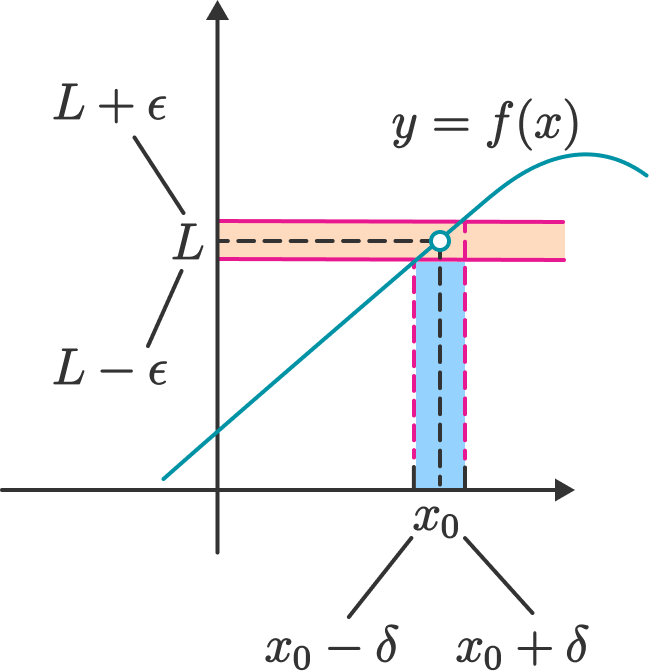
\includegraphics[width=4cm]{edlimit.png}
\end{center}
What the epsilon delta definition of a limit approaching $x_0$ is saying in terms of this picture is simply $L$ is our limit if for a chosen epsilon, delta exists where my interval on the $x$-axis gives values of $x$ where $f(x)$ is within epsilon of $L$. This probably still makes your head hurt/spin and it probably won't stop. However, let'd make more sense of this with some examples. Let's show this is true by this definition.
$$\ds\lim_{x\rightarrow 3}4x-5=7$$
Let's just plop this into our definition.
$$|x-3|<\delta, \hspace{1cm} |(4x-5)-7|<\epsilon.$$
Simplify and find our left inequality!
$$|(4x-5)-7|=|4x-12|=4|x-3|<\epsilon \Rightarrow |x-3|<\dfrac{\epsilon}{4}.$$
If we take $\delta=\dfrac{\epsilon}{4}$ we have proved this!\\
Let's try another.
$$\ds\lim_{x\rightarrow 3}x^2=9$$
Once again plop in.
$$|x-3|<\delta, \hspace{1cm} |x^2-9|<\epsilon.$$
Let's do some simplifying.
$$|x^2-9|=|(x-3)(x+3)|<\epsilon.$$
Thus, we need to bound the $x+3$! Then we are home free!
Since we are looking at $x$ as we approach 3, in particular, $x$ close to 3; let's use a distance of 1 from 3! Therefore, $|x+3|<7$ for $2\leq x\leq 4$. Delta with be smaller than this so we are ok! Over this interval, we also have $|x-3|<1$. Let's see what happens when we use this.
$$|(x-3)(x+3)|<7|x-3|<\epsilon\Rightarrow |x-3|<\dfrac{\epsilon}{7}.$$
\textbf{OR} we can just use $|x-3|<1$. Thus, $\delta$ should be the smaller of the 2 of these. Namely, $\delta=\min\lbrace 1, \dfrac{\epsilon}{7}\rbrace$.\\
THIS IS HARD! Please practice!\\\\
Continuity- We discussed this lightly in class, but we know a function is continuous at $a$ if the limit is the same as $f(a)$. This brings up the idea of discontinuity. When we seek continuity we are really looking for an $x$ such that we do not have this condition! Examples include holes, piecewise functions, 'jumps', and asymptotes. A nice property of continuous functions is that you can move the limit inward for a cont. function. What does this mean? Let's look at the function $x^2$. This function is continuous for all $x$. Thus, any limit of this can be represented as the following: $\lim x^2=(\lim x)^2$. This is possible as long as the function is continuous at the limit point! Try looking at general sets of functions and seeing if they are continuous. For example: polynomials, rational functions, complex functions, trig functions, inverse trig functions, etc. This brings us to the big theorem here; The Intermediate Value Theorem!\\ If $f$ is continuous on $[a,b]$ and $N$ between $f(a)$ and $f(b)$ not equal, then there is a $c$ in $(a,b)$ such that $f(c)=N$. \\
We should always ask, so what? An example can tell you why this is valuable.\\
Show the following has a root.
$$4x^3-6x^2+3x-2$$
Something, say $c$, is a root if $f(c)=0$. The Intermediate Value Theorem is a picking something bigger and something smaller than 0 means I have a $c$ for which this is true since this polynomial is continuous! To save time and computation, $f(1)=-1$ and $f(2)=12$. Thus, somewhere between 1 and 2 there is a $c$ for which $f(c)=0$! Done! Notice we did not find the root, but we know it exists.\\\\
Inifinte limits- I talked about these briefly as an exercise in class. I mentioned that the big technique is to divide by the highest power of $x$ in your function for rational functions. There are more techniques such as multiplying by the conjugate and the dividing by largest power with respect to a root. You do need to be careful!\\
I mentioned lightly in class that dividing by the highest power has a discrepency in math. In this class it seems you will need to divide by the highest power in the \textbf{denominator only}. The idea is the following: 
$$\ds \lim_{x\rightarrow \infty}\dfrac{x^2}{x}=\ds \lim_{x\rightarrow \infty} x=\infty$$
BUT if we do divide by $x^2$ everywhere we get a 0 denominator which is undefined!\\
Lastly, if $\ds\lim_{x\rightarrow\pm\infty} f(x)=L$ then $y=L$ is a horizontal asymptote. i.e. draw a line here and the graph of the function approaches this line in but does not touch it in the direction of infinity or negative infinity accordingly. 
\newpage
\begin{enumerate}[1.]
\item Prove the following via epsilon delta:
\begin{enumerate}[a.]
\item $\ds\lim_{x\rightarrow1}\dfrac{2+4x}{3}=2$
\item $\ds\lim_{x\rightarrow-2}x^2-1=3$
\item $\ds\lim_{x\rightarrow2}x^3=8$
\end{enumerate}
\item Determine if the function is continuous. If it is not, give all the discontinuous points.
\begin{enumerate}[a.]
\item $\begin{cases} 
      x+1 & x\leq 1 \\
      \dfrac{1}{x} & 1< x< 3 \\
      \sqrt{x-3} & x\geq 3 
   \end{cases}$
   \item $\begin{cases} 
      x+2 & x< 0 \\
     e^x & 0\leq x\leq 1 \\
      2-x & x>1 
   \end{cases}$
\end{enumerate}
\item Prove the folllowing have a root on the interval given by IVT.
\begin{enumerate}[a.]
\item $\sqrt[3]{x}=1-x$, (0,1)
\item $\sin(x)=x^2-x$, (1,2)
\end{enumerate}
\item Find the limits or show they do not exist ( $\pm \infty=DNE$).
\begin{enumerate}[a.]
\item $\ds\lim_{x\rightarrow\infty}\dfrac{(2x^2+1)^2}{(x-1)^2(x^2+x)}$
\item $\ds\lim_{x\rightarrow\infty} \dfrac{\sqrt{9x^6-x}}{x^3+1}$
\item $\ds\lim_{x\rightarrow -\infty} x+\sqrt{x^2+2x}$
\end{enumerate}
\item Sketch the graph given the following: $\ds\lim_{x\rightarrow 2}f(x)=\infty$, $\ds\lim_{x\rightarrow-2^+}f(x)=\infty$, $\ds\lim_{x\rightarrow-2^-}f(x)=-\infty$, $\ds\lim_{x\rightarrow-\infty}f(x)=0$, $\ds\lim_{x\rightarrow\infty}f(x)=0$, and $f(0)=0$.
\end{enumerate}
\end{document}







